\section{Introduction}
\label{sec:introduction}

The laboratory assignment presented has for its purpose the study of a circuit
structured in four elementary meshes, through which exist seven resistors $R_i$,
a voltage source $V_a$, a current controlled voltage source $V_c$, a current
source $I_d$ and a voltage controlled current source $I_b$. The circuit can
be seen in Figure-\ref{fig:circuit}.


Throughout the report it is presented a theoretical analysis, a simulation of the
circuit and its analysis as well as a comparison of the obtained results. \par
In Section~\ref{sec:analysis},  both mesh and nodes methods are applied, in order to do
a theoretical analysis of the circuit, using the Octave maths tool.
In Section~\ref{sec:simulation}, it is executed an analysis of the circuit using
the Ngspice tool to simulate it. Lastly, in Section~\ref{sec:conclusion}, it is
performed a comparison between the results from both the theoretical analysis
and the simulation, from Section~\ref{sec:analysis} and Section~\ref{sec:simulation},
respectively.


\begin{figure}[H] \centering
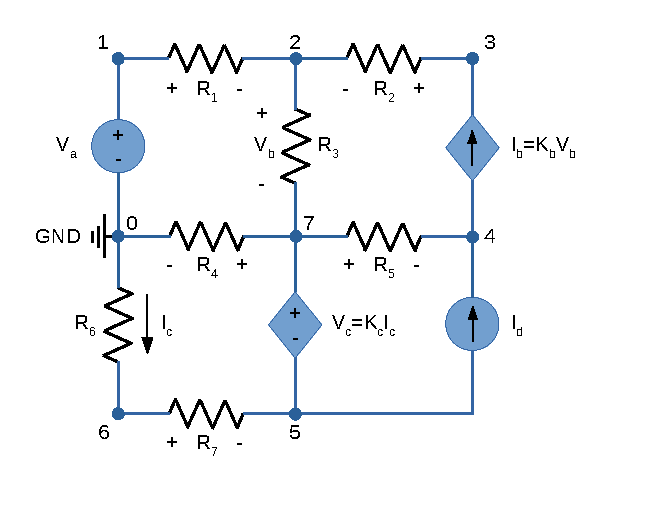
\includegraphics[width=0.7\linewidth]{circuit.pdf}
\caption{Circuit.}
\label{fig:circuit}
\end{figure}

